\documentclass{article}
\usepackage{parskip}
\usepackage{pdfpages}
\usepackage[margin=.6in]{geometry}
\begin{document}
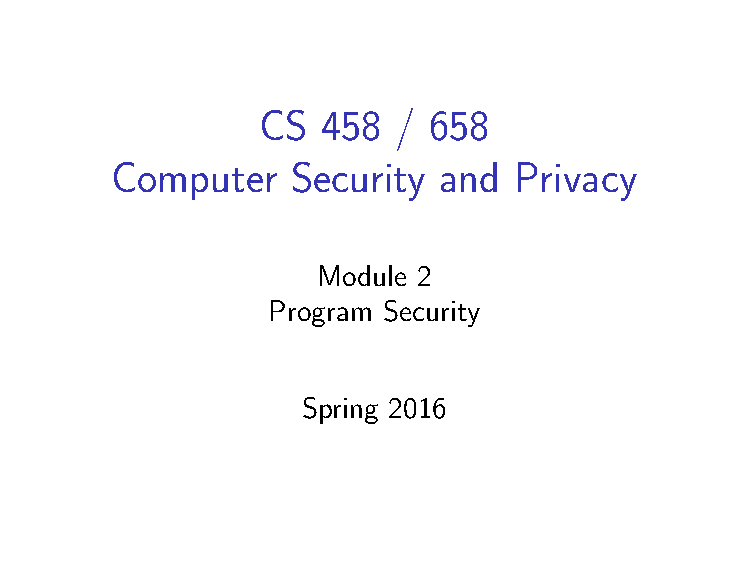
\includepdf[page=1-18]{Module2.pdf}

\section{Heartbleed} % (fold)
\label{sec:heartbleed}
Happened when people could request data of a given length where the length does not match the length of the data requested so they get more data than they are authorized to. In heartbleed you could use this to get the servers encryption key to decrypt all traffic on a server. To fix this all you have to do is have a bounds check when data is requested. If its wrong ignore the request because obviously they are lying. Heartbleed started more people looking at ssl and people found tons of errors in openssl. 
% section heartbleed (end)

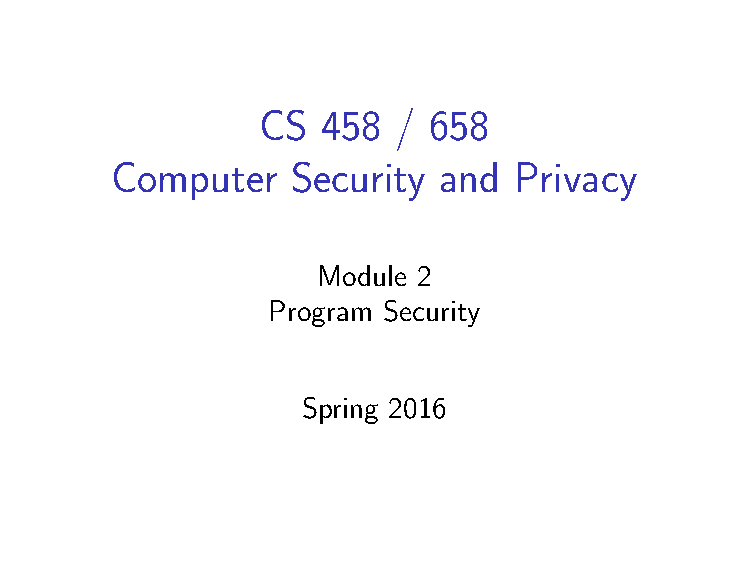
\includepdf[page=19-21]{Module2.pdf}
\section{Apple's SSL} % (fold)
\label{sec:apple_s_ssl}
This was caused by a really stupid error where there was two gotos without brackets around them causing the second one to never execute. This could have been detected by code reachability tests. It was named the hashtag goto fail. 
% section apple_s_ssl (end)

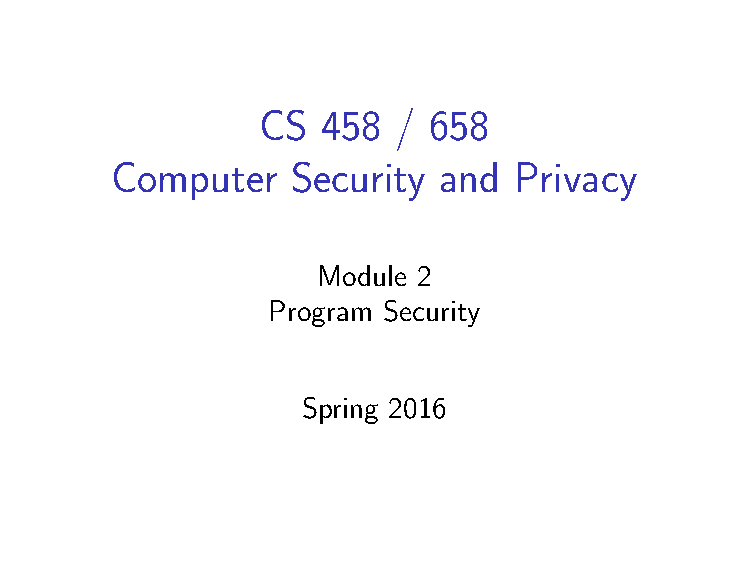
\includepdf[page=22-24]{Module2.pdf}
\section{Buffer Overflow} % (fold)
\label{sec:buffer_overflow}
When you initialize a buffer you give it a length, when you try to add more data to that buffer than it has length for it starts trying to write that data around the buffer. This normally accidentally tries to overwrite critical data causing a segfault. If the attacker is smart enough and knows the layout of the program they can abuse this. Usually the code about where to jump to is written in the stack, so if they can use a buffer overflow to access those values they can make your code jump to their executable causing them to gain access to your stuff. Usually java will throw an out of bounds exception to protect this. This causes a crash of the program if you don't catch it. This causes your shit to go down which is BAD. Most buffer overflow attacks are nearly impossible because lots of languages and programs have catches built in to stop them so in real life this is ridiculously hard to do. This course uses a VM to let them overwrite these fail safes.

Common attack points are set uid programs. This happens when a thins ownership has \texttt{rwsr--r--}. The s means that the set uid flag is set allowing it to set the user type.

(all ordering goes from highest address to lowest address here) The stack loads the main program into the highest addresses, then it loads any necessary programs (like a function you call from main) below it. Within that frame on the stack is the return address for that function call. At the top of a frame is the parameters, then return address, then frame pointer, then local variables. When we make an array it goes in the local variables. The array starts with a[0] at the lowest address and grows up. If we go past the array bounds it will allow us to write into the frame pointer of this frame (since this was the next thing up on the stack). If we keep going we can eventually overwrite the return address. We can use this to jump to shell code that allows us to run anything. 

Important to note that there are other variables that can change the flow of the program, you have to overwrite these as well.

If you put a ton of NOPs in your "shell" you can make it much larger so that its easier to hit the shell program. You should be using gdb instead to get the exact address of things instead of blindly guessing and hoping for the best.
% section buffer_overflow (end) 

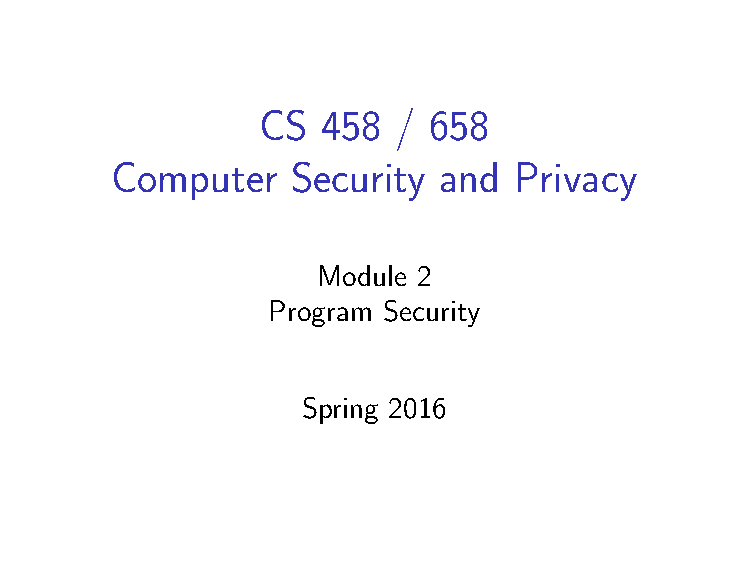
\includepdf[page=25]{Module2.pdf}
\section{Kinds of Buffer Overflows} % (fold)
\label{sec:kinds_of_buffer_overflows}
A common cause of buffer overflows are off by one errors. Another kind is to use buffer overflows to return to another part of the program (called \textbf{Return Oriented Programming}). For instance to skip over a check for the password or such. The super cool cutting edge one is \textbf{Blind Return Oriented Programming} which is a deamon that continuously tries things. Basically is a tool that can get a buffer overflow without knowing anything about the program.
% section kinds_of_buffer_overflows (end)

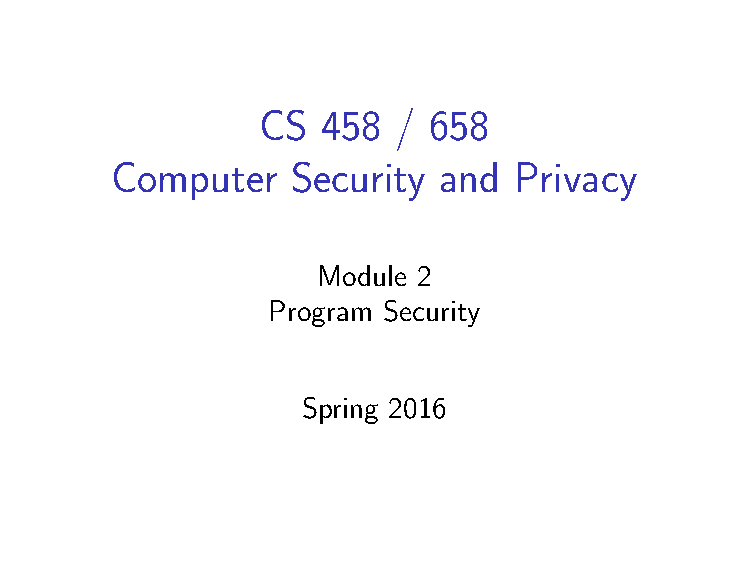
\includepdf[page=26]{Module2.pdf}
\section{Defense} % (fold)
\label{sec:defense}
There is a defense that says that cannot write to a program and execute it (only one or the other) called \textbf{W NAND X}. ROP is a way around this. Another one is \textbf{Address Space Layout Randomization} which keeps changing where in memory stuff is stored so that you cannot use your knowledge of the layout of the memory to do buffer overflows since stuff is always in a different place. Doesn't work too well on 32bit because theres isn't enough randomization so you can get around it by running your program over and over. Lastly is \textbf{Canaries} that detect if the stack has been overwritten.
% section defense (end)
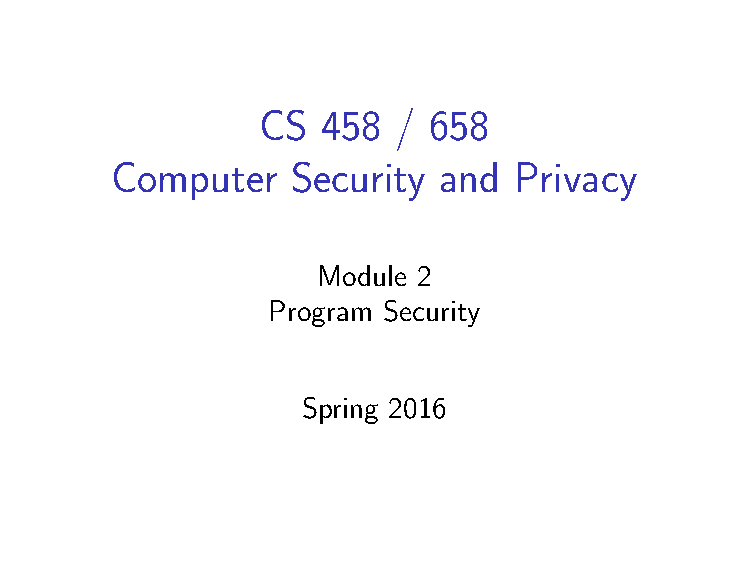
\includepdf[page=27]{Module2.pdf}
\section{Integer Overflows} % (fold)
\label{sec:integer_overflows}
Basically this is caused by someone casting an unsigned integer to a signed integer causing the value of the number of bypass what you expected it to be.
% section integer_overflows (end)

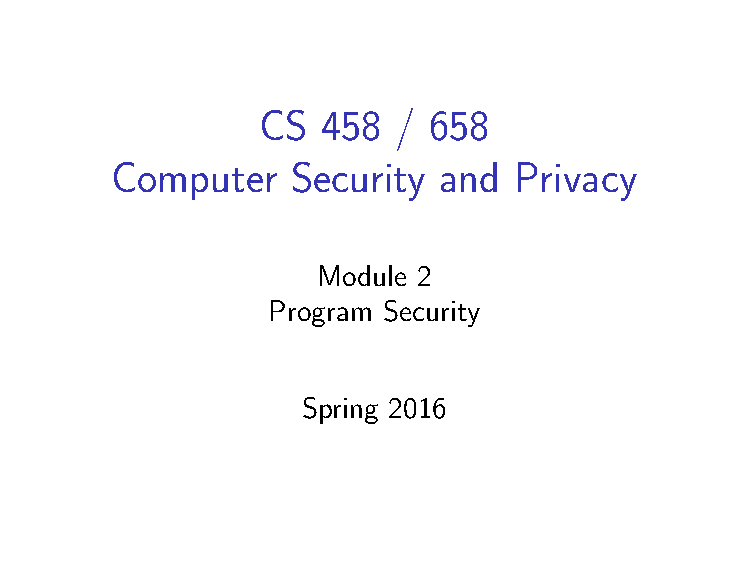
\includepdf[page=28]{Module2.pdf}
\section{Format String Vulnerabilites} % (fold)
\label{sec:format_string_vulnerabilites}
You can use this to read past what is accessible memory. So if your print format doesnt have proper parameters for it it will keep looking for something to print allowing the program to print stuff that probably should not have been printed. \texttt{print("\%s")} will die in a fire because it is looking for something to print causing it to segfault. You can use \%x to print parts of the stack or \%n to know how much has been printed. 

For example: When you call printf it will read the format string until it finds a variable which causes it to look that value up in the stack frame. It then bumps up what it is looking for in the stack to print. If you don't provide enough variables for its format string it will look up in the stack the next thing. After each variable read the printf bumps up its stack pointer which is what tells it where to look if a variable isn't provided. 
% section format_string_vulnerabilites (end)

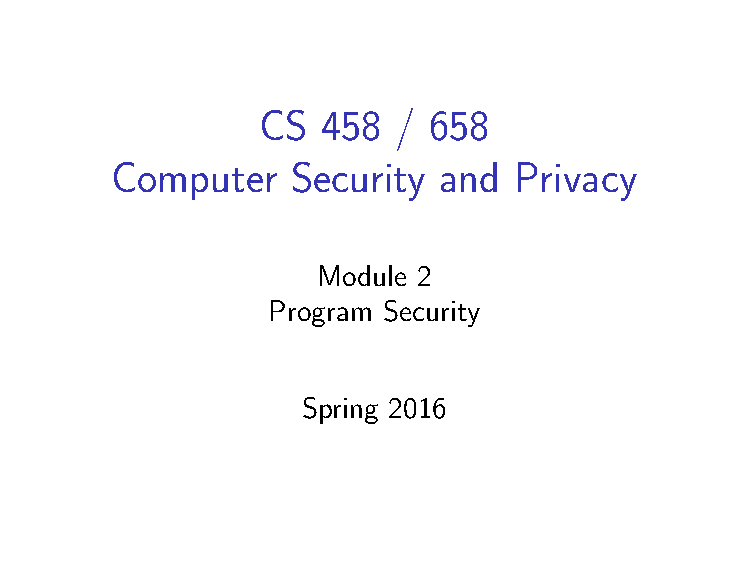
\includepdf[page=29-37]{Module2.pdf}
\section{Incomplete Mediation} % (fold)
\label{sec:incomplete_mediation}
This is when the user input can fuck shit up. We don't know much about the users that might just be really stupid. Malicious user can fuck up your database if you don't check for stuff.Frequently forms will use hidden fields to remember information about the user, more commonly they use cookies. These are very public facing things, anyone with a browser debugger can find this data and manipulate what is sent in these special fields.

You can sign the stuff you send to the backend to sure that you acknowledge that you actually did this. The more common way is to use sessions that makes the data expire.

% section incomplete_mediation (end)
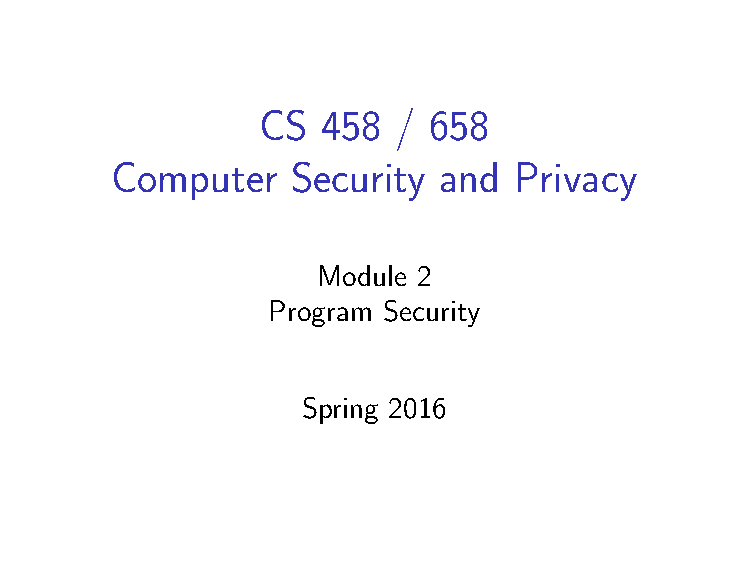
\includepdf[page=38-41]{Module2.pdf}
\section{TOCTTOU Errors} % (fold)
\label{sec:tocttou_errors}
The user asks the system if it is allowed to perform an action then lets it do that. If there is some time between when it checks for permission and actually doing the action you can sneak in and change the permission. You can increase the amount of time by giving the code a very large file to read or such. This means that the attacker can almost always win the race.

You can work with file handles instead of names (these are returned when you call fopen, the computer makes a table of lookups for files). File handles cannot be changed once you open them to prevent them pointing you to a different file. Locks are also your friend, they can prevent another thread from sneaking in while you are checking permission.
% section tocttou_errors (end)

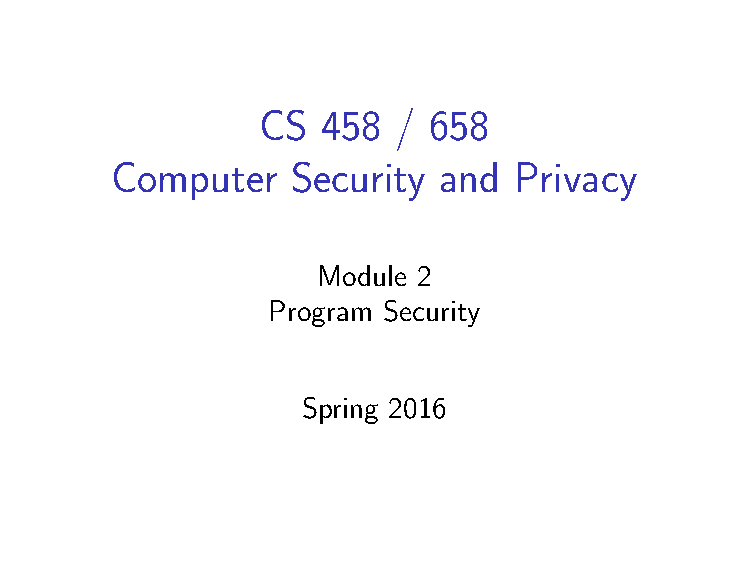
\includepdf[page=43-48]{Module2.pdf}
\section{Malware} % (fold)
\label{sec:malware}
You cannot do anything with downloaded malware, it must be executed. You want to try to exploit a flaw in the system to cause it to execute automatically. Viruses are a kind of malware with a payload they want to execute on their system. They tend to try to be super stealthy so they often insert themselves into a executable, so that when it is run it runs itself and then the host virus. Usually you cannot just append yourself to the start of a program due to addressing and such. You want to add your virus to the end, copy the first instruction below the virus, then replace the first instruction with a jump to your virus. Viruses will try to spread itself. Particularly when the user shares files.

Historical examples:
\begin{itemize}
	\item creeper(1971)
	\item cloner(1982)
	\item brain(1986) - infected PCs
	\item stoned(1987)
	\item ping pong(1988)
\end{itemize}

% section malware (end)

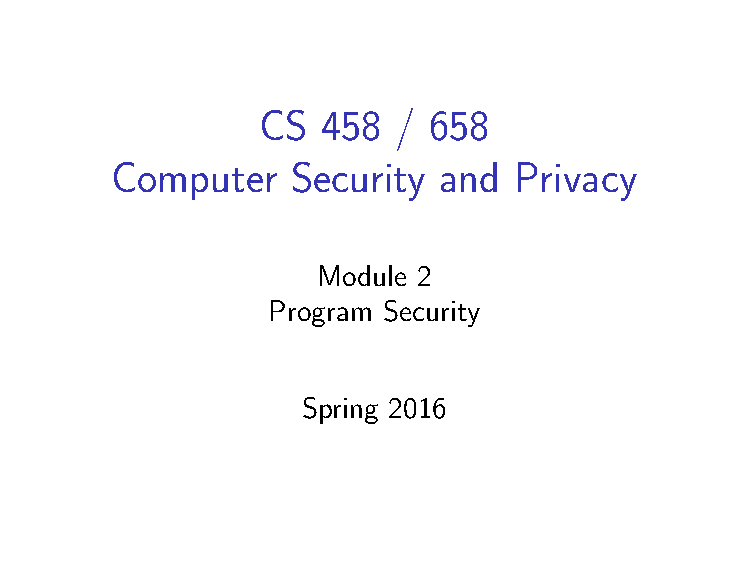
\includepdf[page=49-52]{Module2.pdf}
\section{Catching Viruses} % (fold)
\label{sec:catching_viruses}
	
Spotting a virus is very hard. One way is applying a signature to files that watching for it. The signature you can catch virus payloads and patterns of a virus. The problem is that you can avoid signature based virus spotters by using polymorphism. You can encode your virus and frequently change the key for it. You have an decryption key, then decryption code, then encrypted malware code. To catch these you can look for the decryption code is common amongst all copies of the virus so you can look for it.

Instead of looking at what the virus looks like you can watch for its behaviour. Problem is you have run them first to see what it does. Commonly this is done in a sandbox and see what it does. Of course viruses now can look to see what environment it is running in and behaves nicely when it does.

% section catching_viruses (end)

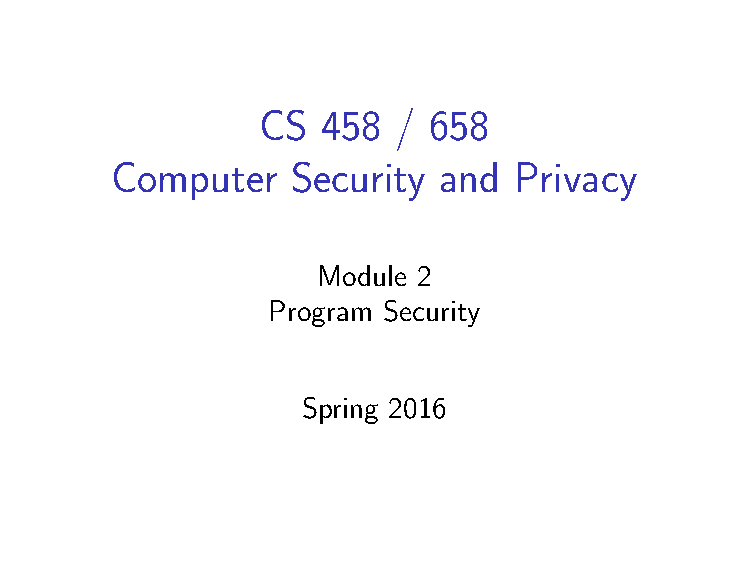
\includepdf[page=53]{Module2.pdf}
\section{False Positives and Negatives} % (fold)
\label{sec:false_positives_and_negatives}
	
It almost always better to have false negatives since they are mildly annoying but not harmful to the user. The flip side is you can get warning fatigue where the user gets so sick of you false positive shit that they no longer listen to warnings leaving them completely open to all viruses.

In a signature based system it is possible to have false positives, but you really shouldn't if you are programming it properly. False negatives are much more possible, especially with new software the system hasn't see before. In behaviour based systems are prone to false positives, they can also have false negatives.
% section false_positives_and_negatives (end)

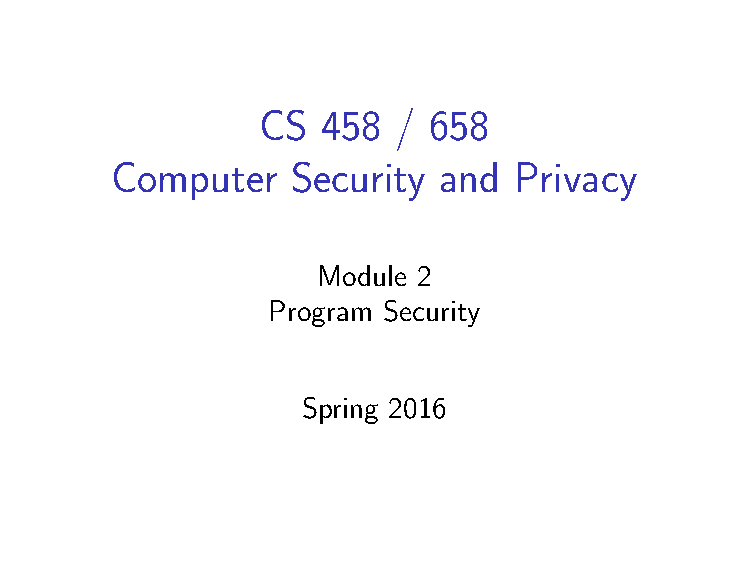
\includepdf[page=54]{Module2.pdf}
\section{Base Rate Fallacy} % (fold)
\label{sec:base_rate_fallacy}
Based on this example, say we have 50 people for whom the system says you're drunk but aren't, this means that there is 1 actual drunk (this is out of 1000 people). Leading to 51 drunk results. If you get a positive result there is 1:51 chance that you actually are drunk. This means that the system is pretty useless.
% section base_rate_fallacy (end)

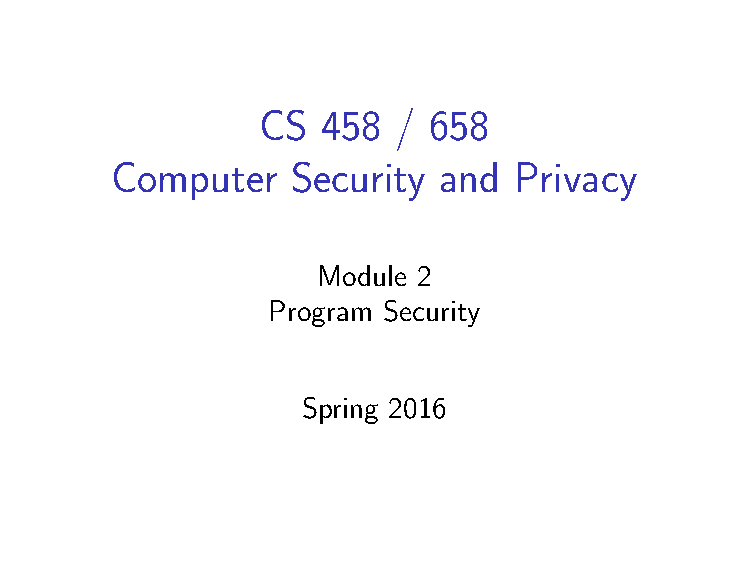
\includepdf[page=55-58]{Module2.pdf}
\section{Trojan Horses} % (fold)
\label{sec:trojan_horses}
These look like they do something helpful when actually they want to wreck your shit. This gets the user to run the code. You have to make them want it, you aren't tricking them into running it on accident. Also known as Potentially Unwanted Programs (called PUPs).
% section trojan_horses (end)

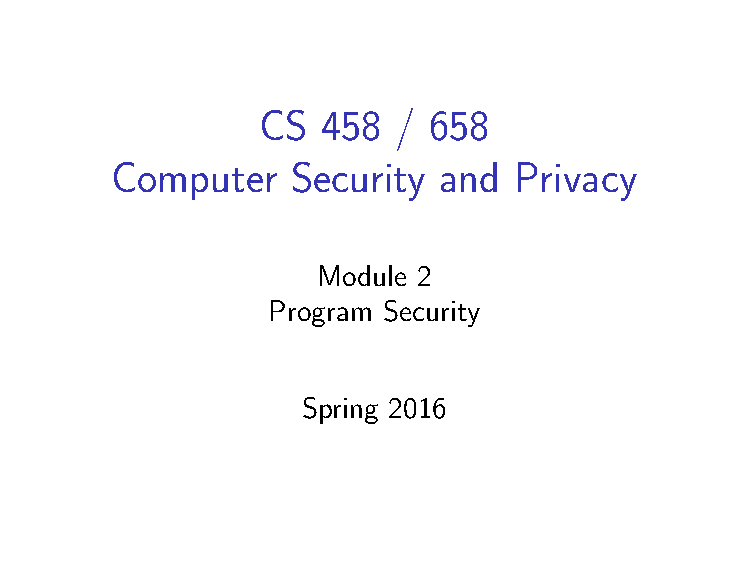
\includepdf[page=59]{Module2.pdf}
\section{Scareware} % (fold)
\label{sec:scareware}
These scare us into installing or running stuff in order to prevent viruses. These are the actual viruses

% section scareware (end)

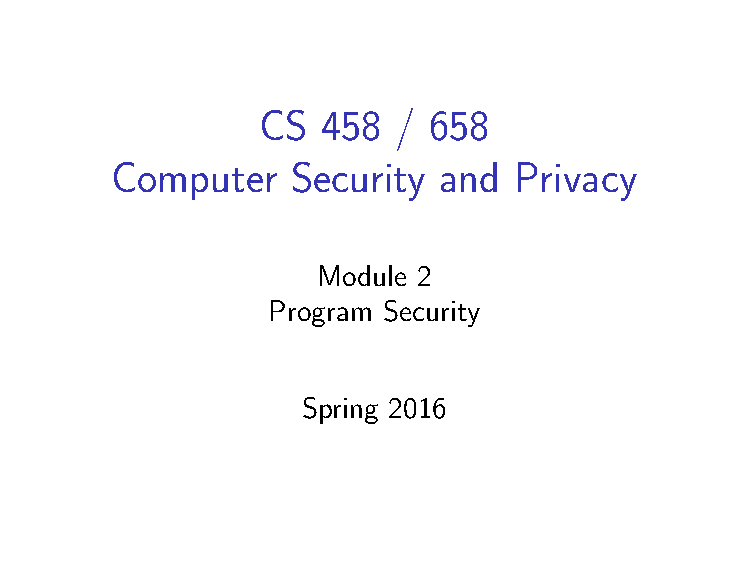
\includepdf[page=60-61]{Module2.pdf}
\section{Ransomware} % (fold)
\label{sec:ransomware}
Basically this locks up your computer until you agree to pay them some sum to unlock it. CryptoLocker is a famous one the the FBI shut down. Another one shut down a full hospital.
% section ransomware (end)

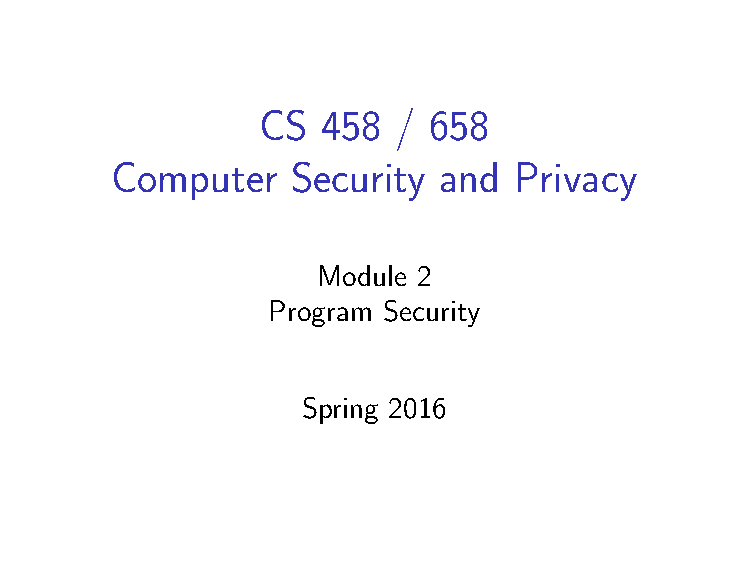
\includepdf[page=62-64]{Module2.pdf}
\section{Logic Bombs} % (fold)
\label{sec:logic_bombs}
This code doesn't do anything for a long time, or until some trigger occurs. An example is something placed on a system by someone that knows they are going to be fired soon. Another example of this is an easter egg, which isnt malicious. Trojan horses are often logic bombs as well. This makes checking for them a lot harder. 
% section logic_bombs (end)

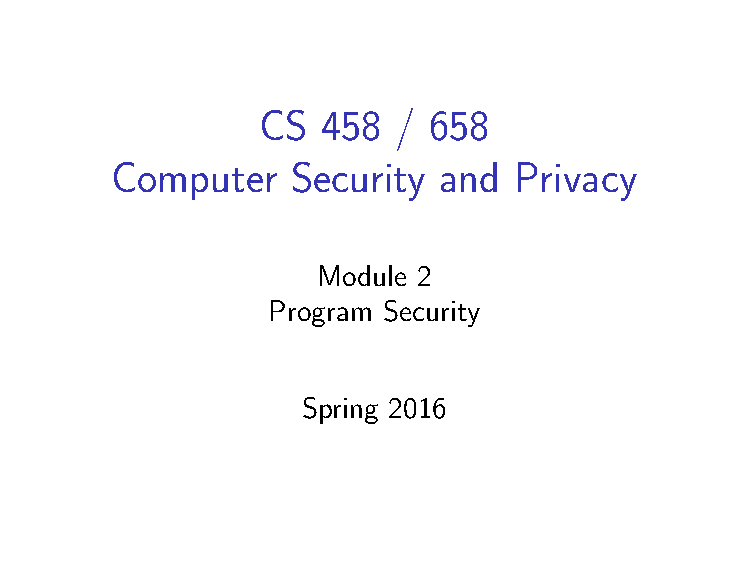
\includepdf[page=65-71]{Module2.pdf}
\section{Worms} % (fold)
\label{sec:worms}
Worms are essentially bits of code that can replicate itself. The Morris worm is the most famous example where a guy put a thing on Myspace that got him friends and duplicated itself. Stuxnet abused 0 day vulnerabilities which are vulnerabilities that no one knows about. A common theory is that stuxnet and flame were developed by the government.

\begin{tabular}{|c|c|c|}
	\hline
	& \textbf{Virus} & \textbf{Worm}\\
	\hline
	\textbf{payload} & yes & sometimes\\
	\hline
	\textbf{distribution} & requires user interaction & spreads by itself\\
	\hline
	\textbf{location} & attached to exe's & standalone\\
	\hline
	\textbf{self-replicating} & yes & yes\\
	\hline
\end{tabular}
% section worms (end)

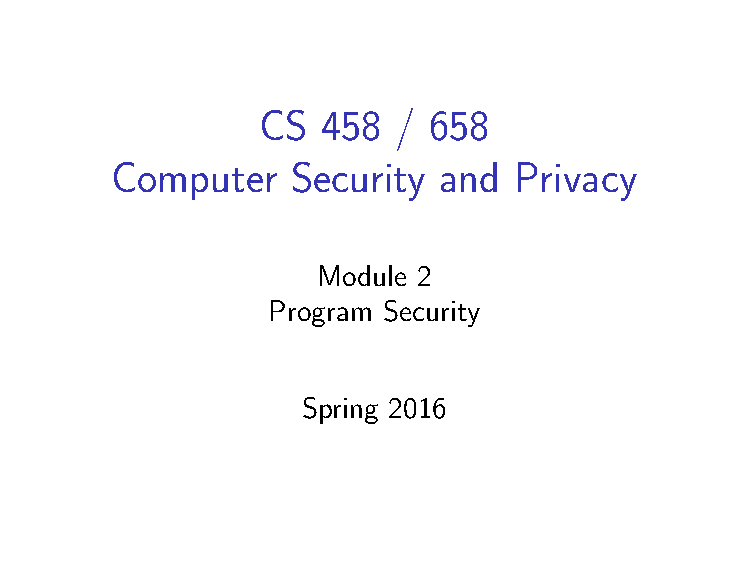
\includepdf[page=73-76]{Module2.pdf}
\section{Web Bugs} % (fold)
\label{sec:web_bugs}
These are secret things that cause you browser to connect to a third party server. Usually a single pixel image or iframe. They can use this to get your ipaddress or store information in cookies. When you first go somewhere with a web bug it places a cookie on your browser so that when you go other places it can request that cookie and link where you've gone. Frequently this is used as adds to generate analytics about you. Addblock tends to just remove the adds and not let them load. When you follow a link it can send an HTTP referrer. When you're on a site you follow a plain old link and your browser provides some information about where you just came from. 

These allow websites to send all of this information everywhere without your permission. Defences for this are disabling cookies on your browser which can suck. You can also periodically delete all of your cookies. You can also just disable third party cookies. 

% section web_bugs (end)

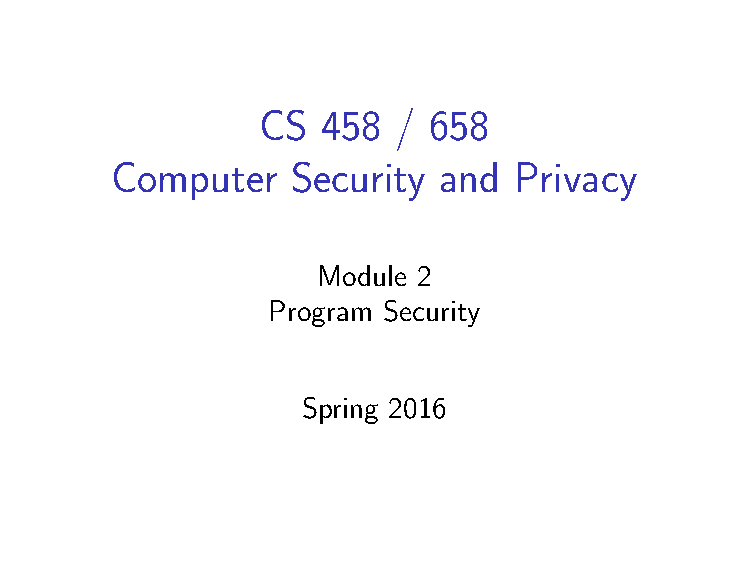
\includepdf[page=77-82]{Module2.pdf}
\section{Back Doors} % (fold)
\label{sec:back_doors}
These are things added to the software that lets people get access to your software without your permission. Frequently they are used for debugging or testing, just make sure you remove them before shipping. In the example from this linux kernel there is a check that accidentally sets the user to root instead of checking if it is root. Another example is port knocking where a accessing a specific pattern of ports will give root access. Wake on LAN is listening for a specific pattern that will cause it to wake up.

Juniper Networks dual EC incident was discovered in dec 2015 but it was added in 2012, this was a baackdoor in their routers which are used by many big companies. There were actually 2 back doors. One was an authentication bypass which was a simple backdoor in the password checker. The other was was a backdoor in its pseudo-random number generator. There is a system parameter called Q which is supposed to be chosen randomly. If the hacker knows some value P where Q = f(P) they can predict the outcome of the random number generator even if they don't know the seed. 

% section back_doors (end)
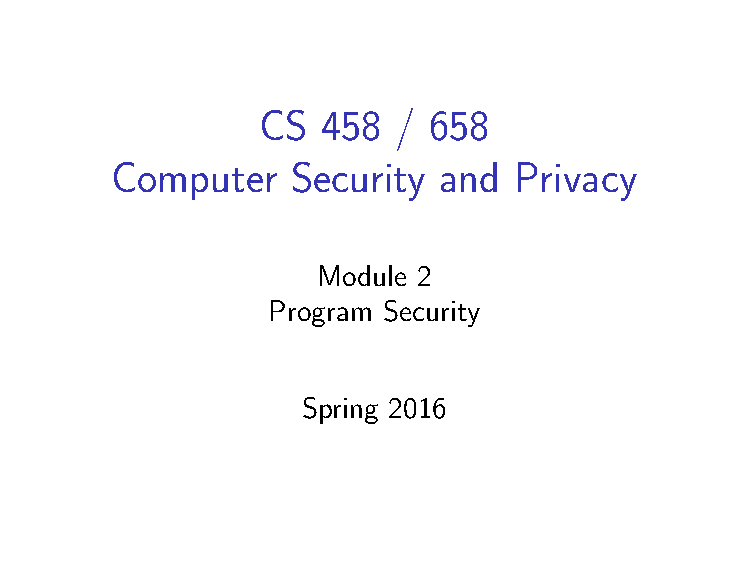
\includepdf[page=77-82]{Module2.pdf}
\section{Salami Attacks} % (fold)
\label{sec:salami_attacks}
We have a bunch of small things that do a tiny amount of damage in each attack so that people consider it inconsequential. In hackers they save the bits of cents that get rounded off and transfer them into their account. 
% section salami_attacks (end)

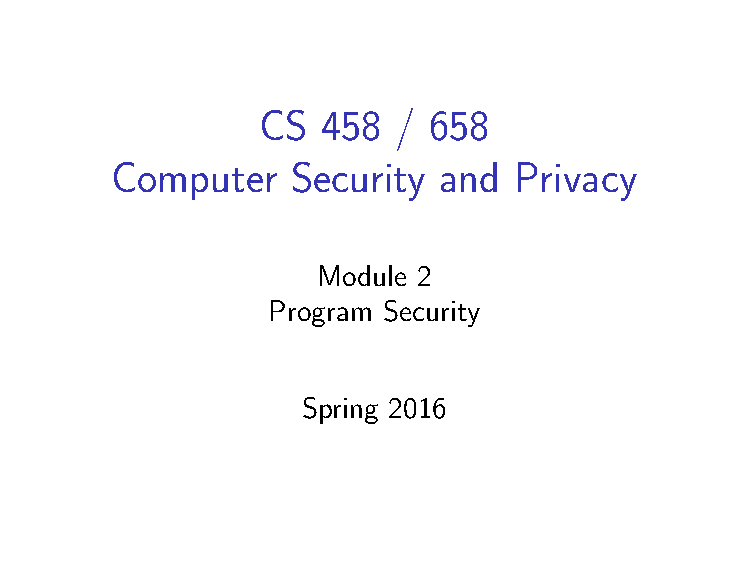
\includepdf[page=84-85]{Module2.pdf}
\section{Privilege Escalation} % (fold)
\label{sec:privilege_escalation}
This is when you have some privileges and you escalate them to gain more access. Most of the previously mentioned attacks try to achieve this (like sql injection, buffer overflows, etc). A froot attack has some user connecting to a root machine and they type \texttt{telnet machine userid} so the telnet sends the userid through to the machine. That machine executes \texttt{rlogin userid}. This prompts for a password and so on. There is a argument \texttt{-f} that lets you bypass the password check if you are the root user already. So the attacker can send \texttt{telnet machine -froot} this gets sent as if the user name was \texttt{-froot} the machine executes the command which works because the telnet demon on the machine is running as root so the -f makes it not ask for a password and logs you in as root. There are only 3 characters not allowed in unix usernames: null characters, colons, and new lines.
% section privilege_escalation (end)

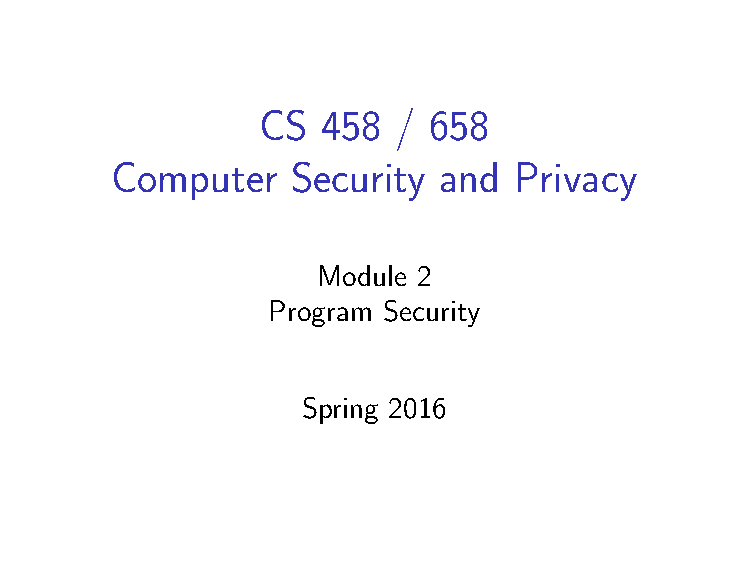
\includepdf[page=86-89]{Module2.pdf}
\section{Rootkits} % (fold)
\label{sec:rootkits}
These are little tools to get you root privileges for you. It often hides itself, by removing entries in log files, modifying commands to hide themselves (ls and ps), or modifying the kernel so that it doesn't show these files. 

An example is a guy that was developing a thing to scan rootkits on a machine. He eventually found that he had a rootkit on his machine that came from a sony media disk. This was intentional from Sony to keep people from copying disks. It named all of its files with a special prefix that it then modified shit to ignore that. Lots of people abused this by naming their malware with that same suffix so that their malware would be hidden as well. Sony was forced to release a uninstaller that also left a backdoor. 
% section rootkits (end)

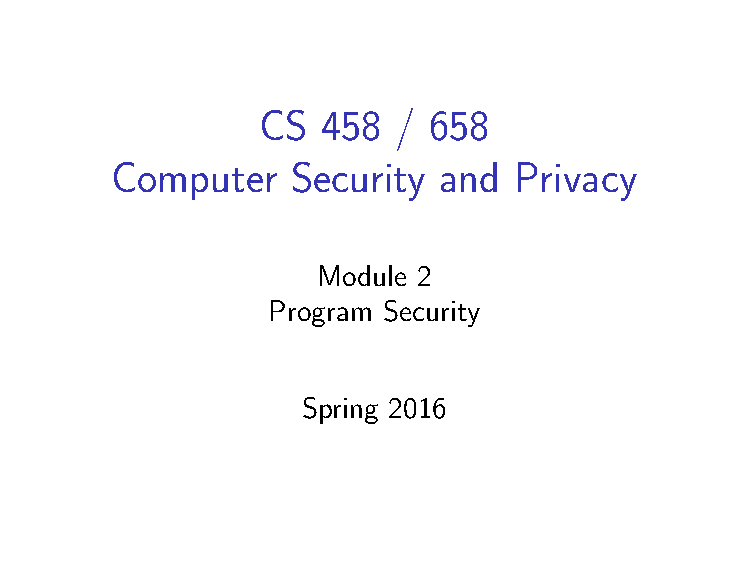
\includepdf[page=90-92]{Module2.pdf}
\section{Keystroke loggers} % (fold)
\label{sec:keystroke_loggers}
Basically these just log every key stroke that happens on your machine. You can actually just buy these from reputable companies. These can be hardware ones (you just plug a keyboard into it and it into the computer).
% section keystroke_loggers (end)

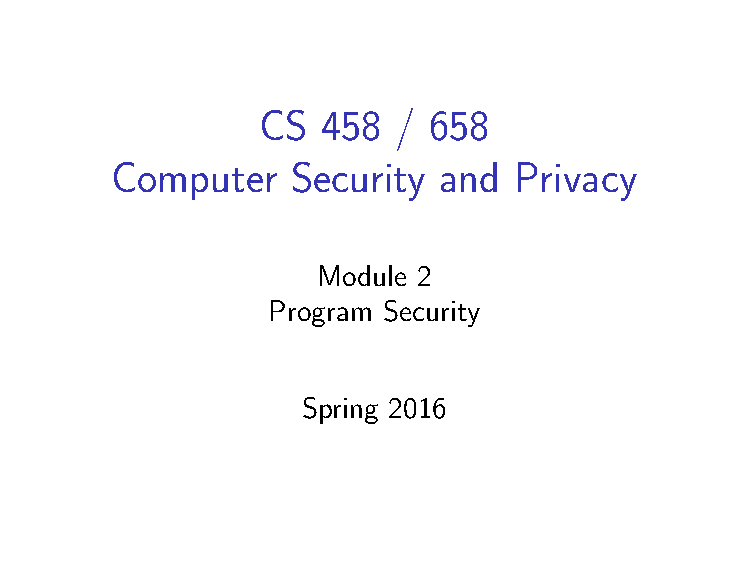
\includepdf[page=93-96]{Module2.pdf}
\section{Interface Illusions} % (fold)
\label{sec:interface_illusions}
These are things that look almost identical to what you'd expect but don't do what you think. For example a scroll bar that is also secretly a button to move some malware into your startup folder. Another example is conficker where the autorun dialog on a usb that creates a run command that looks identical to the open folder icon that encouraged the user to run your shit. \textbf{Clickjacking} is another thing where a user goes to click on a button that they think is legit, but in actual fact it is overlayed on top of something else that is much more nefarious. This makes the click go through to the underlying shitty button. 

Another example of this is phishing. Where you think you are going somewhere legit but you arent. Now url bars must use fonts that distinguish between all characters (so l I 1 are different). Some phishers from just tunnel into the legit sight so all of the information is correct. The word phishing comes from phone hacking. Lots of people were making false phone calls called phreaking, so they stuck with it.
% section interface_illusions (end)

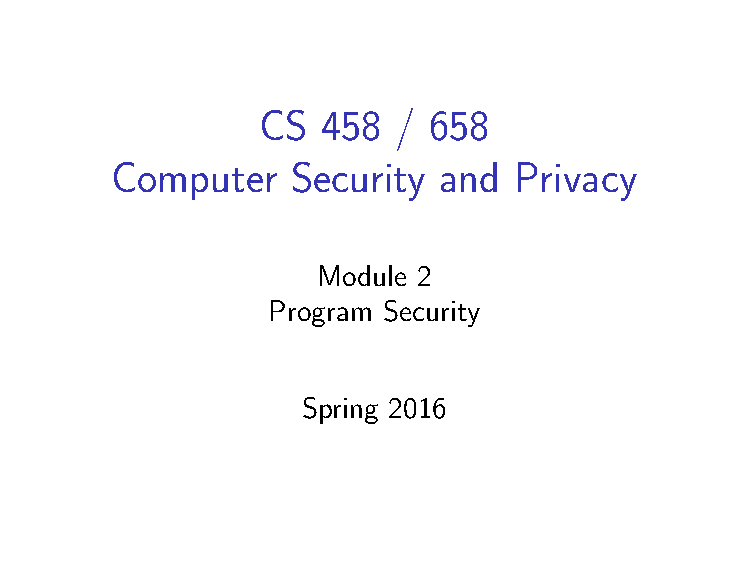
\includepdf[page=97-98]{Module2.pdf}
\section{Man-in-the-Middle} % (fold)
\label{sec:man_in_the_middle}
These are just attacks where someone sits in between the user and their endpoint and manipulates the data going though. Interface illusions are a good example of this.
% section man_in_the_middle (end)

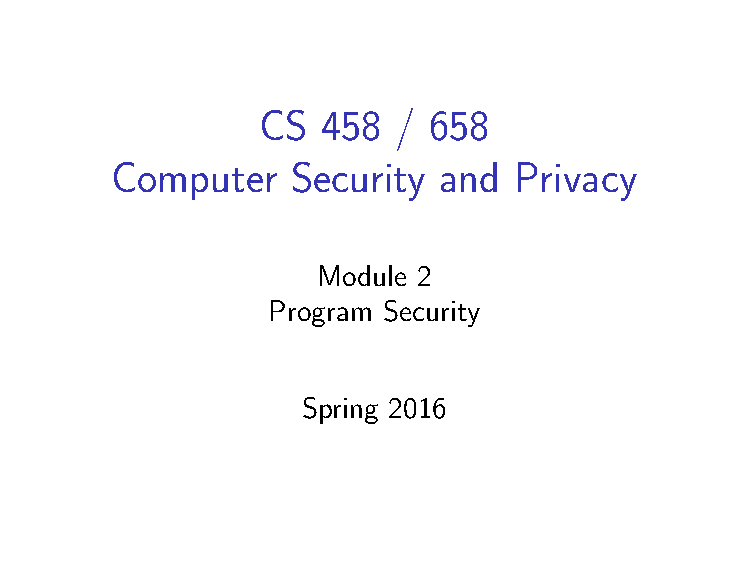
\includepdf[page=100]{Module2.pdf}
\section{Cover Channel} % (fold)
\label{sec:cover_channel}
This is hiding data within something else. Steganography is a method for encoding information in unusual places. A common version is to hide information in packets going over the network not in its packet but in unused headers. 
% section cover_channel (end)

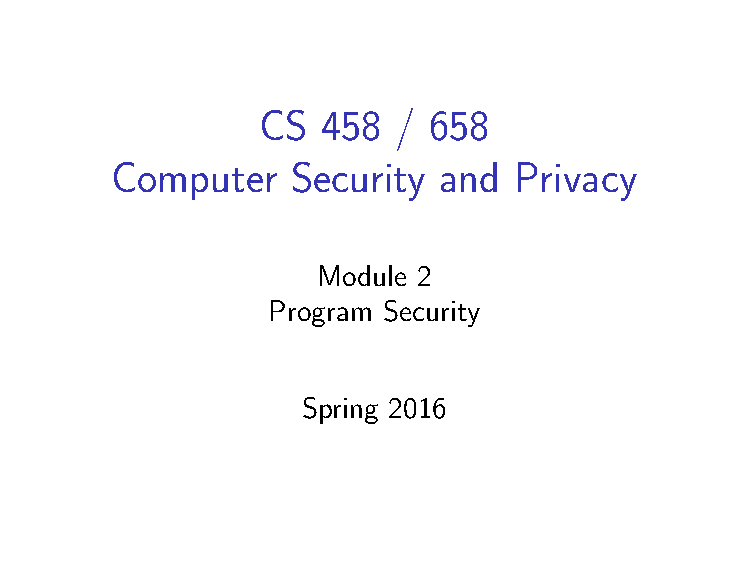
\includepdf[page=101-102]{Module2.pdf}
\section{Side Channel} % (fold)
\label{sec:side_channel}
These are when a user is accidentally leaking data. Some people figured out how to recode the whine of a cpu to figure out what calculations its doing. Holy shit! A more common one is to monitor power usage. You can do timing side channel in square-and-multiplying to compute $x^d$ mod n. d is a secret represented in binary. For each 0 its one multiplication and for each 1 it is two. You can run statistical analysis on timings to figure out what d is. 

% section side_channel (end)

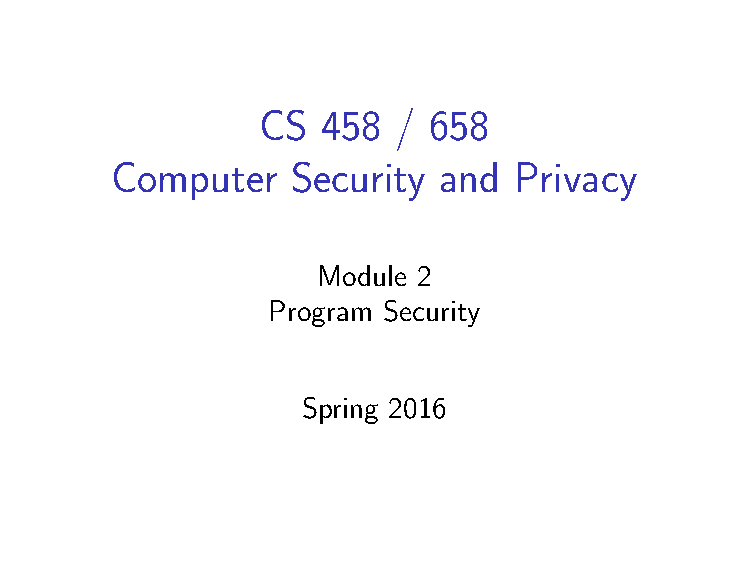
\includepdf[page=105-110]{Module2.pdf}
We can help make shit way more secure by just using good coding practices, encapsulation and modularity for example.

Mutual suspicion basically just means don't trust anyone, even yourself. Sanitize all data and authenticate everything. This also falls under the term mediation.

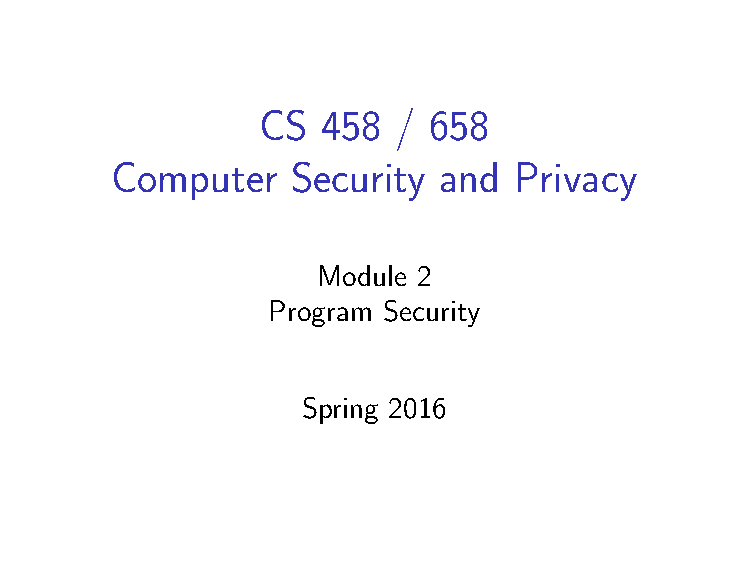
\includepdf[page=111]{Module2.pdf}
You can confine your data by limiting what access it has. This is a bit like mutual suspicion but for a specific module. This increases overhead as you have to validate tons of stufff for that program. Its good to do with very sketchy data.








\end{document} 